\section{Theoretical Background}
\label{sec:theoretical_background}

\subsection{Shrinkage and Sparsity}
\label{subsec:shrinkage_and_sparsity}
The topic of both shrinkage and sparsity is related to parameter regularization where the researcher sacrifices a little bias to reduce the model variance \parencite{tibshirani_regression_1996}. This is also commonly referred to as the bias-variance trade-off which describes the dilemma of finding a balanced trade-off between model complexity and model fit. Typically, a complex model with many parameters has a smaller bias and a higher variance in comparison to a less complex model with fewer parameters. In the case of a linear regression model, the predictive error depends on both the bias and the variance. In forecasting scenarios, one is typically interested in a model which generalizes well to new data. This means that overly complex models lead to poor predictive performance due to an inflated variance while too simple models lead to poor predictive performance due to a larger bias \parencite[pp.~223~f.]{hastie_elements_2009}.

A common way to address the bias-variance trade-off is through parameter regularization in the form of shrinkage and/or sparsity. Shrinkage refers to shrinking certain parameter estimates towards zero by penalizing large values. Sparsity refers to setting certain parameter estimates to exactly zero which leads to excluding them from the model at all. Both techniques aim at the same goal -- reducing the predictive variance while sacrificing bias \parencite{figueiredo_adaptive_2003,tibshirani_regression_1996}.

A popular example for both shrinkage and sparsity is the lasso regression model first introduced by \citeauthor{tibshirani_regression_1996} in \citeyear{tibshirani_regression_1996}. It extends the standard ordinary least squares (OLS) optimization problem by adding a penalization term for the absolute parameter values called the $L_1$-norm. The $L_1$-constrained least squares optimization problem for a regression model $y = X \beta + \epsilon$ with $p$ parameters can be written as
\begin{align}
    \label{eq:lasso_optimiziation_problem}
    \text{arg} \min_{\beta} \; \underbrace{(y - X\beta)' (y - X\beta)}_{\text{Sum of squared residuals}} + \underbrace{\lambda \sum_{j = 1}^{p}|\beta_j|}_{L_1\text{-penalization}} \; \text{,}
\end{align}
where $\lambda \geq 0$ controls the strength of shrinkage \parencite{park_bayesian_2008,yuan_efficient_2005,tibshirani_regression_1996}.

In Bayesian inference, shrinkage and sparsity can be implemented through the choice of adequate prior distributions. For the lasso example, one can show that a Bayesian regression model with a Laplace prior on the coefficients centered at zero yields the frequentist lasso estimate at the posterior mode (proof in Appendix~\ref{app:bayesian_lasso_estimate}). The general intuition behind centering the prior at zero is to assume a priori that the coefficients are likely to be close to zero. This also pulls the coefficients' posterior distributions to zero if the evidence in the data does not show otherwise.

To illustrate how the choice of a prior shrinks posterior estimates an empirical example has been conducted. The task was to predict the horsepower of cars in R's default \emph{mtcars}\footnote{\url{https://www.rdocumentation.org/packages/datasets/versions/3.6.2/topics/mtcars}} dataset based on information such as fuel consumption or weight. Figure \ref{fig:bayesian_lasso_parameters} shows the coefficients' posterior distributions for each regressor used to predict car horsepower.
\begin{figure}[h]
    \centering
    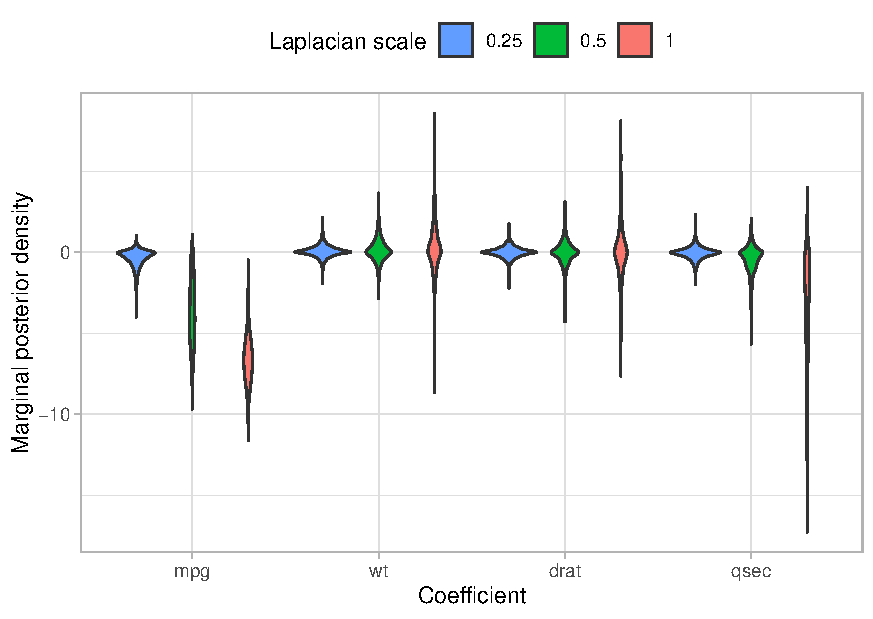
\includegraphics[width=0.75\textwidth]{figures/bayesian_lasso_parameters.pdf}
    \caption{Posterior distributions for parameter estimates grouped by different Laplacian scale parameters.}
    \label{fig:bayesian_lasso_parameters}
\end{figure}
One can observe that smaller Laplacian scale parameters lead to stronger shrinkage. This reflects the fact that smaller scale parameters lead to a sharper Laplace prior distribution with more probability mass around zero which pulls the posterior estimates to zero as well.

This specific example leads to both a shrunk and a sparse model. The posteriors of \emph{wt} (weight) and \emph{drat} (rear-axle ratio) show strong evidence that both regressors have little explanatory power because the distributions have most probability mass around zero. A point-estimate like the posterior mode becomes close to or exactly zero which effectively excludes the regressors from the model. With increased shrinkage, the same behavior can be observed for \emph{qsec} (quarter-mile seconds). Finally, \emph{mpg} (miles per gallon) seems to be the most important regressor to predict horsepower because its posterior distributions are strongly different from zero even for increased shrinkage.

\subsection{Vector Autoregressive (VAR) Models}
\label{subsec:var_model_defintion}
Vector autoregressive (VAR) models can be used to model multivariate time series. They gained popularity in the macroeconomic field after the influential paper by \textcite{sims_macroeconomics_1980}. This section defines VAR models following the notation of \textcite{hauzenberger_combining_2021}.

A VAR($p$) model with $p$ lags has the following form:
\begin{align}
    \label{eq:var_model_definition}
    y_t = A_1 y_{t - 1} + \dots + A_p y_{t - p} + C + \epsilon_t \; \text{,}
\end{align}
where $y_t = (y_{1t} , \dots , y_{mt})'$ represents an $m$-dimensional vector of observations at time $t = 1 , \dots , T$. $A_j$ for $j = 1 , \dots , p$ is the ($m \times m$) matrix of coefficients at the $j$'th lag of $y_t$. The model's intercept is denoted by the ($m \times 1$) vector $C$. Finally, $\epsilon_t \sim \mathcal{N}(0, \Sigma)$ is the Gaussian shock vector with mean zero and $\Sigma$ as its ($m \times m$)-dimensional variance-covariance matrix.

Furthermore, define $\alpha = vec\{(A_1, \dots , A_p , C)'\}$ as the vector of vectorized coefficients which has dimension $k = m (mp + 1)$ and $x_t = (y_{t - 1}' , \dots , y_{t - p}' , 1)'$ as the $(n = pm + 1)$-dimensional vector of explanatory variables. With these definitions at hand it is possible to rewrite Equation~\eqref{eq:var_model_definition} as a regression model
\begin{align}
    y_t = (\mathcal{I}_m \otimes x_t') \alpha + \epsilon_t \; \text{.}
\end{align}

Another form of notation commonly found in literature is the full matrix notation of VAR models \parencite{koop_bayesian_2009}. Define $A = (A_1 \dots , A_p , C)'$ and $E$ as $(T \times m)$-dimensional matrix of stacked shocks with $t$th row $\epsilon_t'$. With $t$th row $y_t'$ in $Y$ and $t$th row $x_t'$ in $X$ the matrix notation reads
\begin{align}
    Y = XA + E \; \text{.}
\end{align}

A bivariate $(m = 2)$ VAR model with one $(p = 1)$ lag can be written as follows:
\begin{align}
    \begin{pmatrix}
        y_{1t}\\
        y_{2t}
    \end{pmatrix}
    =
    \underbrace{
        \begin{pmatrix}
            a_{11} & a_{12}\\
            a_{21} & a_{22}
        \end{pmatrix}
    }_{m \times m}
    \underbrace{
        \begin{pmatrix}
            y_{1t-1}\\
            y_{2t-1}
        \end{pmatrix}
    }_{m \times 1}
    +
    \underbrace{
        \begin{pmatrix}
            c_1\\
            c_2
        \end{pmatrix}
    }_{m \times 1}
    +
    \begin{pmatrix}
        \epsilon_{1t}\\
        \epsilon_{2t}
    \end{pmatrix}
    \; \text{.}
\end{align}
This instance of the simplest possible VAR model already has $6$ coefficients and $4$ variance-covariance values to be estimated which underlines the fact that VAR models suffer from a fast-growing number of parameters. This issue, which is also referred to as the curse of dimensionality, motivates the upcoming contents of this seminar paper, which address this problem by describing shrinkage and sparsification techniques for VAR models.
